\documentclass[a4paper, 11pt]{article}
\usepackage{comment} % enables the use of multi-line comments (\ifx \fi) 
\usepackage{lipsum} %This package just generates Lorem Ipsum filler text. 
\usepackage{fullpage} % changes the margin
\usepackage{enumitem}
\usepackage{qtree}
\usepackage{amsmath}
\usepackage{amsfonts}
\usepackage{algorithm}
\usepackage[noend]{algpseudocode}
\usepackage{graphicx}

\makeatletter
\def\BState{\State\hskip-\ALG@thistlm}
\makeatother

\begin{document}
%Header-Make sure you update this information!!!!
\noindent
\large\textbf{Individual Design Journal 6} \hfill \textbf{Basil R. Yap} \\
%\normalsize ECE 100-003 \hfill Teammates: Student1, Student2 \\
2018 -- Capstone 7 \hfill Journal Date: 2018/06/21 \\
Project 61: Steelcase \hfill Due Date: 2018/06/17

\section*{Problem Statement}

All work regarding the \textit{Container Loading Optimization (CLO)} problem is going according to plan and a functional prototype is expected to be complete in time for \textbf{Review 3}.\\

As covered in the previous Journal (\textbf{Journal 5}), the \textit{CLO} Problem has been broken down with consideration to the usability of the algorithm with respect to the management team at Steelcase Malaysia as well as members of the public during the Capstone Showcase.

Therefore, the work completed by me over the last few weeks are as follows, in chronological order:
\begin{enumerate}
\item Benchmarking of existing 3D-bin packing algorithms
\begin{enumerate}
\item Literature review \& Implementation (continued)
\item Algorithm scoring \& Test results
\end{enumerate}
\item Visualisation of algorithm solutions
\begin{enumerate}
\item Feasibility testing of conventional visualisation tools
\item Preliminary design of web application \& UI *
\item Front-end development iterations
\end{enumerate}
\end{enumerate}

\textit{* not covered in this Journal.}

\section*{Benchmarking of existing 3D-bin packing algorithms}

\subsection*{Literature review \& Implementation}

Upon further research into the problem of 3D-bin packing, a list of algorithms were compiled and implemented. The following are the algorithms we have finalised and completed, accompanied by a short description on their respective packing strategies:\begin{enumerate}
\item S-Pack / H1 \cite{Martello}\\

S-Pack considers the problem by dividing the bin into layers. Each layer is filled in order from the back of the bin to the front using 2D-bin packing algorithms. Each layer's 2D-bin area depends on the 3D dimensions of the boxes arranged in prior layers.
\item MPV-BS / H2 \cite{Martello}\\

MPV-BS is a branch-and-bound method where only $m$ branches were considered at each node. The tree search space exponentially increases with more classes of box sizes, therefore, a hyperparameter was set in order to limit the search space of the algorithm. Based on the paper's experimental results, $m=4$ was selected.
\item Height first - Area second (HA) \cite{HA}\\

Height first - Area second is a straight forward heuristic, where the bin was loaded from a corner with priority given to boxes with the tallest height and ties were broken with priority given to boxes with the largest area.
\item Extreme point best fit decreasing \cite{Extreme}\\

Extreme point best fit decreasing is a combination of two heuristics, extreme point and best fit decreasing. Extreme point selects the locations to consider for box placement, while best fit decreasing gauges the \textit{merit} of the box placed in that location. The bin is iteratively filled from back to front by assigning boxes (if any) with the highest \textit{merit} score at every extreme point.
\end{enumerate}

\subsection*{Algorithm scoring \& Test results}

For testing, the following parameters were used in the test algorithm, as shown in \textbf{Algorithm 1}:
\begin{itemize}
\item Bin size: 1190 x 228 x 219 (\textit{SMM's 40ft Container Size})
\item Number of Boxes generated: 200
\item Box size range (width, height, depth): [73, 119] (\textit{min/max of current box size})
\item Number of Box size classes: [1, 6]
\item Number of Repeat tests: 100
\end{itemize}

\begin{algorithm}
\caption{Test Algorithm}
\begin{algorithmic}[1]
\Procedure{TestProcedure}{n}
\State $\text{noBox}\gets200$
\State $\text{batch}\gets\lfloor\text{noBox}/n\rfloor$
\State $\text{bin}\gets(1190,228,219)$
\State $\text{dimMin}\gets73$
\State $\text{dimMax}\gets119$
\State $\text{repeat}\gets100$
\State $\text{boxList}\gets\text{Array}[\mathbb R]$
\State $\text{solutionArray}\gets\text{Array}[\mathbb R^2]$
\For{$i=1$ to repeat}
	\State $\text{noBox}\gets200$
	\While{$\text{noBox}>0$}
	\If{$\text{noBox}\geq(2\times\text{batch})$}
		\State $\text{noBox}\gets\text{noBox}-\text{batch}$
		\State $\text{boxObj}\gets$ \Call{randBox}{dimMin, dimMax}
		\For{$j=1$ to batch}
			\State boxList \textbf{append} boxObj
		\EndFor
	\Else
		\State $\text{boxObj}\gets$ \Call{randBox}{dimMin, dimMax}
		\For{$j=1$ to noBox}
			\State boxList \textbf{append} boxObj
		\EndFor
		\State $\text{noBox}\gets0$
	\EndIf
	\EndWhile
	\For{$f(x,y)\in$ algorithmSet}
		\State arrangedSet $\gets f$(bin, boxList)
		\State failedSet $\gets$ \{boxList\}\textbackslash\{arrangedSet\}
		\State solutionArray[$f(x,y)$][i] $\gets$ \Call{Count}{failedSet}
	\EndFor
\EndFor
\For{$f(x,y)\in$ algorithmSet}
	\State solutionArray[$f(x,y)$] $\gets$ \Call{Average}{solutionArray[$f(x,y)$]}
\EndFor
\Return{solutionArray}
\EndProcedure
\end{algorithmic}
\end{algorithm}

The results of the test can be seen graphically in \textbf{Figure 1.}\\

Experimentally, Extreme Point performed the best across all box size classes.\\
It performed on average 7\% better than S-Pack, which was the worst algorithm overall.

\begin{figure}[h!]
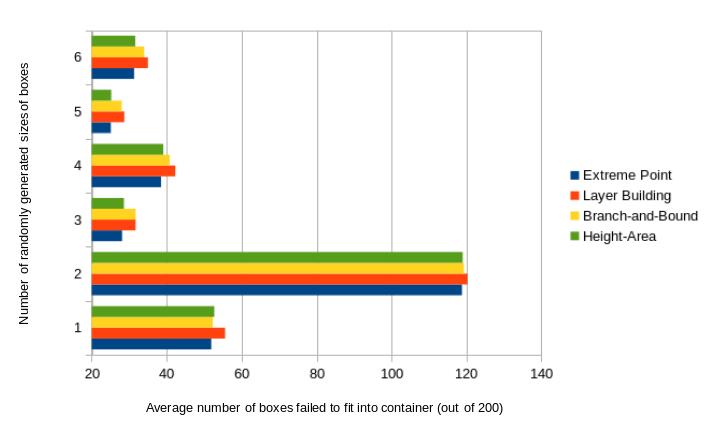
\includegraphics[width=\linewidth]{./assets/201806271010.png}
\label{figure:figure1}
\caption{Benchmark Test Results}
\end{figure}

\pagebreak

\section*{Visualisation of algorithm solutions}

\subsection*{Feasibility testing of conventional visualisation tools}

Upon completion of the algorithms, the focus turned towards finding a suitable way of visualizing the solutions generated. The solution consists of a "list" object, where each box has the following two attributes:\begin{itemize}
\item reference id: a unique identifier to help keep track of the boxes
\item coordinates: the arranged coordinates of the centroid of the box
\end{itemize}

Using a sample solution, we testing the functionality of the following software and implementation languages:\begin{itemize}
\item Microsoft Excel
\item R Language (3dplot, ggplot \& plotly)
\item Python (matplotlib, vtk \& plotly)
\item Tableau \& PowerBI
\end{itemize}

Most of which resulted in the same problem, the visualisations do not convey the information provided by the solution sufficiently well. Due to the limitations of the 3D projection onto 2D space, the relative positions of the boxes are not retained. Also, in cases where the number of boxes/layers are numerous, the overlap of points make the whole visualisation completely infeasible.\\
It is, however, worth noting that a web application created using plotly in R or Python allows the user to turn the plot to provide sufficient navigation of the information. The web application created was still much to be desired as the solution was shown as points and customization was heavily limited by the extents of the Python package.\\

With the success of a simple web application, I decided that a full on web application would be better suited for the task and more fitting as a prototype to be shown to our industry partners.

\subsection*{Front-end development iterations}

The following were some considerations when developing the GUI. All milestones were set using the software development principle of \textit{version control}.

\begin{enumerate}
\item[\textbf{v1.xx}] Establish initial 3D environment
\begin{enumerate}
\item[\textbf{v1.03}] Complete lighting and axis
\item[\textbf{v1.05}] Spawn movable boxes
\item[\textbf{v1.11}] Complete control panel for box generation  
\end{enumerate}
\item[\textbf{v2.xx}] Set-up controls for boxes and bins
\begin{enumerate}
\item[\textbf{v2.02}] Complete controls for bulk spawn of boxes
\item[\textbf{v2.03}] Create permanent 3D estimate of bin size
\end{enumerate}
\item[\textbf{v3.xx}] Interface between algorithm and GUI
\begin{enumerate}
\item[\textbf{v3.01}] Add control panel option for algorithm
\item[\textbf{v3.02}] Test simple python API using Flask
\item[\textbf{v3.05}] Functional prototype for one algorithm
\end{enumerate}
\end{enumerate}

\begin{thebibliography}{9}
\bibitem{Martello} Martello, S., Pisinger, D., \& Vigo, D. (2000). The three-dimensional bin packing problem. \emph{Operations Research}, \emph{48}(2), 256-267.
\bibitem{Extreme} Crainic,T. G, \& Perboli, G., \& Tadei, R. (2007) Extreme Point-Based Heuristics for Three-Dimensional Bin Packing. \emph{INFORMS Journal on Computing}, \emph{20}(3). 368 - 384.
\bibitem{HA} Lodi, A., Martello, S., \& Vigo, D. (2002). Heuristic algorithms for the three-dimensional bin packing problem. \emph{European Journal of Operational Research}, \emph{141}(2), 410-420.
\end{thebibliography}

\end{document}
